% Knowledge Graphs - Deliverable 2: first part of project report (max 4 pages without refs as per course)
% CVPR/NeurIPS style: https://github.com/cvpr-org/author-kit/releases
\documentclass[10pt,a4paper]{article}
\usepackage[utf8]{inputenc}
\usepackage[T1]{fontenc}
\usepackage{lmodern}
\usepackage[margin=1.6cm]{geometry}
\usepackage{microtype,booktabs,hyperref,graphicx}
\usepackage[numbers,sort&compress]{natbib}
\usepackage{amsmath,amssymb}
\usepackage{tikz}
\usetikzlibrary{arrows.meta,positioning}
\setlength{\parindent}{0pt}
\setlength{\parskip}{0.38em}
\newcommand{\kteam}{Thalia Delhaise, Lenny Briclet, Andr\'e Fonseca, Rafael Gufler (DL + KG joint project)}

\title{Link Prediction on a Multi-Relational Knowledge Graph:\\
FB15k-237, Matched KGE, and Planned Hard-Negative \& Slice Analysis}
\author{\kteam}
\date{RC2526 --- Deliverable 2 (Report part 1)}

\begin{document}
\maketitle
\thispagestyle{empty}
\vspace{-0.5em}
\subsection*{1.\ Introduction and motivation}
A \textbf{knowledge graph} (KG) is a set of binary facts $(h,r,t)$ over a finite set of \textbf{entities} $\mathcal{E}$ and \textbf{relation types} $\mathcal{R}$. \textbf{Link prediction} (knowledge base completion) asks which missing triples are true: for a query with one side hidden, e.g.\ $(h,r,?)$, rank all candidate tail entities. This is a standard \textbf{learning on graphs} task with applications to semantic query answering and maintenance of large knowledge bases.

In this project we (i) \textbf{materialize} a benchmark KG from the \textbf{FB15k-237} public triple files, (ii) run \textbf{TransE} and \textsc{RotatE} under matched conditions, and (iii) develop \textbf{custom hard-negative} training and \textbf{relation-wise} evaluation---the main methodological extensions. A \textbf{relational GNN} is a \textbf{optional} add-on for the final phase if time allows; it is not required for the core claim.

Our \textbf{contribution} is: reproducible KGE baselines; \textbf{own PyTorch} code for harder negatives and ablations vs.\ defaults; and \textbf{analysis} (slices, error cases) on the \textbf{same} \textbf{filtered} metrics (Hits@$k$, MRR).

\subsection*{2.\ Problem statement}
\textbf{Formal graph.} $\mathcal{G}=(\mathcal{E},\mathcal{R},\mathcal{T})$ with $\mathcal{T}\subseteq\mathcal{E}\times\mathcal{R}\times\mathcal{E}$. The graph is \textbf{directed} and \textbf{multi-relational:} the same node pair can appear in several relations. Training sees only $\mathcal{T}_{\mathrm{train}}$. Validation and test are disjoint held-out \textbf{positive} triples.

\textbf{Data.} \textbf{FB15k-237} (Freebase-derived)~\citep{sun2019rotate}: 14,541 entities, 237 relations, 272,115 / 17,535 / 20,466 training, validation, and test triples. The benchmark is widely used; inverse relations are removed to reduce trivial inferences. We load the official split via \textbf{PyKEEN}~\citep{ali2021pykeen}; optional RDF/edge export for a KG visualization slide is a minor technical step.

\textbf{Task.} \textbf{Link prediction:} for each test triple, rank the correct head or tail under the \textbf{filtered} setting~\citep{bordes2013translating} (candidates that complete a \emph{known} triple in train, val, or test are not errors).

\textbf{Success criteria.} (1)~Strong \textbf{aggregate} filtered MRR and Hits@1,3,10. (2)~Ablations on \textbf{negative} strategies. (3)~Deeper \textbf{relation-wise} and \textbf{degree} analysis and short error study. (4)~\textbf{Optional:} a GNN baseline. We do not claim SOTA; we care \textbf{where} each setting helps or fails.

\subsection*{3.\ Methodology}
\paragraph{Phase A --- Classical KGE (Milestone~1--2).} We implement \textsc{TransE} and \textsc{RotatE}~\citep{sun2019rotate} with PyKEEN for a fair \textbf{first} line: same splits, $d$, optimiser, training budget, and \textbf{filtered} evaluation. The scoring function is learned; training uses margin/ranking loss and negative sampling. This serves as a \textbf{baseline} for the Deep Learning report.

\paragraph{Phase B --- Custom negative mining (in-house PyTorch).} In parallel with KGE, we will implement a \textbf{learnt or scheduled hard-negative} mechanism: e.g.\ a small $g_\phi$ over a subset of corruptions, or periodic \textbf{mining} in embedding space, with ablations \textbf{against} uniform and Bernoulli \textbf{defaults.} This addresses the “not only default PyKEEN” feedback.

\paragraph{Phase C (optional) --- Relational GNN.} If time allows, a shallow \textsc{R-GCN} (or \textsc{CompGCN}) in PyG/DGL~\citep{schlichtkrull2018modeling} on the \textbf{same} task and splits; not required for the main thesis (hard negatives $+$ KGE $+$ analysis).

\paragraph{Evaluation.} In addition to global MRR and Hits@$k$, we will report \textbf{slices} (relation frequency, entity degree) and a short \textbf{error} / case study. Optional bootstrap confidence bands on the test set.

\begin{figure}[h]
\centering
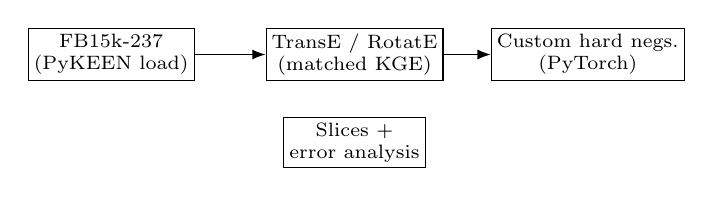
\begin{tikzpicture}[node distance=0.35cm, font=\scriptsize, >=Latex, every node/.style={align=center,draw,inner sep=2pt}]
\node (data) {FB15k-237\\(PyKEEN load)};
\node[right=0.9cm of data] (kge) {TransE / RotatE\\(matched KGE)};
\node[right=0.6cm of kge] (neg) {Custom hard negs.\\(PyTorch)};
\node[below=0.45cm of kge] (slice) {Slices +\\error analysis};
\path[->] (data) edge (kge) (kge) edge (neg);
\path[->] (kge.south) -| (slice.north);
\end{tikzpicture}
\caption{Core pipeline: same filtered evaluation; custom negatives and analysis on the KGE line. GNN (not shown) is optional for later.}
\label{fig:method-kg}
\end{figure}

\subsection*{4.\ Planned experiments and preliminary results}
\paragraph{Planned.} (1)~TransE/RotatE; \textbf{match} $d$ and budget. (2)~Custom negative ablations. (3)~Slice $+$ error analysis. (4)~Optional GNN. (5)~Time/hardware.

\paragraph{Preliminary (Milestone~1).} We use the same training script and protocol as the Deep Learning M1 report (\texttt{code/train\_baseline\_kge.py}): $d=128$, batch 1024, Adam lr $10^{-3}$, up to 15 epochs with early stopping (patience 3) on validation MRR. Test metrics in Table~\ref{tab:prel} are aligned with that report; PyKEEN reports \textbf{realistic} filtered ranking, head and tail prediction averaged (\texttt{both} in PyKEEN's evaluation).

\begin{table}[h]
\centering
\small
\caption{Preliminary aggregate test results, FB15k-237 (same numbers as DL Milestone~1; realistic filtered MRR / H@10, \texttt{both}).}
\label{tab:prel}
\begin{tabular}{@{}lcc@{}}
\toprule
Setting & MRR (filtered) & Hits@10 (filtered) \\
\midrule
TransE        & 0.129 & 0.263 \\
RotatE        & 0.234 & 0.378 \\
GNN (optional)  & --- & --- \\
\bottomrule
\end{tabular}
\end{table}

\subsection*{5.\ Acknowledgment of course deliverables (D2 scope)}
D2 (this document) is the \textbf{first} report slice: \textbf{introduction, problem, methodology, and planned/early results,} to be extended in D3 with full experiments, student contributions, and the Jupyter lab notebook, per RC2526 project text.

\footnotesize
\bibliographystyle{plainnat}
\bibliography{../../shared/references}
\end{document}
